\subsection{Introducción y descripción del algoritmo}

\par Para un primer acercamiento a la solución, buscaremos resolver el problema mediante un algoritmo exacto, es decir, un algoritmo que nos de la solución exacta al problema y no un acercamiento (como veremos mas adelante). En este caso, como no encontramos algoritmos polinomiales que nos brinden la solución al problema, diseñamos un algorítmo de fuerza bruta (backtraking) para ver cómo se comporta y tener un valor exacto de la solución que nos sirva para comparar otros tipos de algoritmos.

\par Un algoritmo de fuerza bruta (o backtraking) se basa en recorrer todas los posibles caminos a la solución hasta encontrarla. El problema en cuestión se trata de encontrar el camino mínimo entre nodos que cumpla ciertas condiciones, por lo que nuestro algoritmo de fuerza bruta recorrerá los nodos de todas las formas válidas (que se cumplan las condiciones pedidas) posibles. A medida que hace esto, irá guardando el mínimo camino conseguido hasta el momento. Cuando finalice todos los caminos posibles podrá asegurar que el camino guardado es el mínimo, ya que recorrió todas las posibles instancias del problema y comparó todos los caminos válidos.

\par Se ve que es un algoritmo simple, se basa en recorrer todas las posibilidades y quedarse con la mejor. El problema se da en que recorrer todas las instancias de un problema suele ser muy pesado. Para algunos problemas, este algoritmo puede ser una herramienta, pero en general, con problemas relativamente grandes (o mejor dicho, no muy acotados), lleva mucho tiempo de computo. Veremos mas adelante que su complejidad aumenta fuértemente en base a algunos parámetros, y esto lo hace muy difícil de correr.

\subsection{Idea general del algoritmo}

\par Previamante contamos que había dos tipos de nodos: gimnasios y paradas. Un jugador puede ir de un nodo a cualquier otro que no haya visitado antes. Por lo que solo nos manejaremos con nodos restantes (los que el jugador aún no visitó) y nodos en el camino (los que sí fueron visitados), y no con enlaces entre ellos (lo que habitualmente se hace cuando se trata de grafos). Entre dos nodos cualesquiera existe una distancia, que calcuaremos al inicio. También es importante notar que para ir a un nodo de tipo gimnasio se debe contar con una serie de pociones. Pero al comenzar el jugador no cuenta con ninguna, por lo que el primer nodo ha visitar siempre debe ser uno del tipo parada.

\par Aclarados estos detalles, retomaremos el ejemplo mostrado en la descripción general del problema (figura \ref{fig: descripcion_ejemplo_entrada}), veremos las distancias entre estos nodos y analizaremos el funcionamiento del algoritmo sobre este caso en particular.

\begin{table}[h]
	\centering
	\begin{tabular}{|>{\centering\arraybackslash}p{2cm}|>{\centering\arraybackslash}p{2cm}|>{\centering\arraybackslash}p{2cm}|>{\centering\arraybackslash}p{2cm}|>{\centering\arraybackslash}p{2cm}|}
		\hline
		   & \textbf{G1} & \textbf{G2} & \textbf{P1} & \textbf{P2} \\ \hline
		\textbf{G1} & \cellcolor{gray} & 1.41421 & 2.82842 & 2 \\ \hline
		\textbf{G2} & 1.41421 & \cellcolor{gray} & 1.41421 & 1.41421 \\ \hline
		\textbf{P1} & 2.82842 & 1.41421 & \cellcolor{gray} & 2 \\ \hline
		\textbf{P2} & 2 & 1.41421 & 2 & \cellcolor{gray} \\
		\hline
	\end{tabular}
	\caption{Distancias entre los nodos del caso de ejemplo.}
	\label{fig: ejercicio1_ejemplo_distancias}
\end{table}

\par En la figura \ref{fig: ejercicio1_ejemplo_distancias} podemos ver las distancias entre los distintos nodos. Vale aclarar que no importa la dirección en la que vaya el jugador, sino los nodos entre los cuales se mueve. Por ejemplo, ir de \textit{P1} a \textit{P2} cuesta 2, igual que ir de \textit{P2} a \textit{P2}.

\par Como comentamos en la introducción, el algoritmo se basa en recorrer los caminos válidos y quedarse con el mejor (mínima distancia). Por lo tanto, al tomar este ejemplo de entrada, el algoritmo comenzará parándose sobre un nodo \textit{i} del tipo parada y calculará todos los caminos posibles partiendo desde él. Luego hará lo mismo para cada uno de los nodos restantes del tipo parada. En el ejemplo, si comienza por el nodo \textit{P1} podrá alcanzar los caminos que se observan en la figura \ref{fig: ejercicio1_ejemplo_caminos1}. En verde están marcadas las distancias mínimas, porque nosotros ya conocemos la solución, pero el algoritmo las toma como mínimo parcial y no sabe aún si van a ser los mínimos generales. Esto porque todavía le quedan por ver todos los caminos que comienzan en el nodo P2.

\begin{figure}[H]
    \begin{subfigure}[b]{0.49\textwidth}
        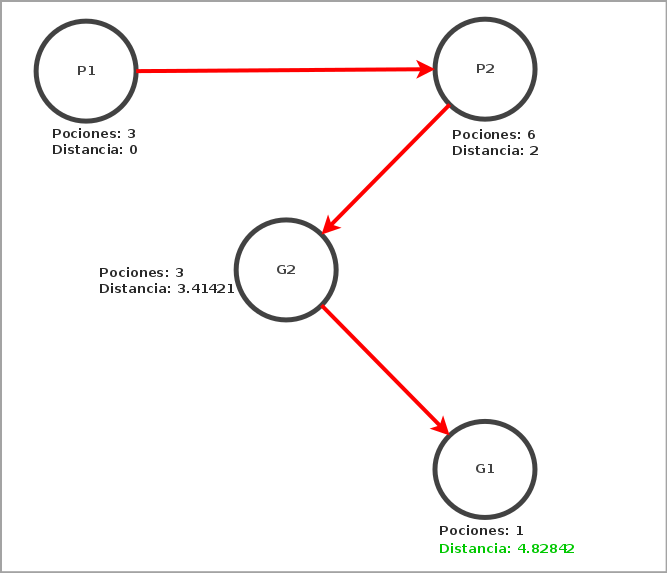
\includegraphics[width=\linewidth]{img/ejercicio1/ejercicio1_ejemplo_camino1_1.png}
        \caption{Camino válido y solución.}
        \label{fig: ejercicio1_ejemplo_camino1_1}
    \end{subfigure}
    \begin{subfigure}[b]{0.49\textwidth}
        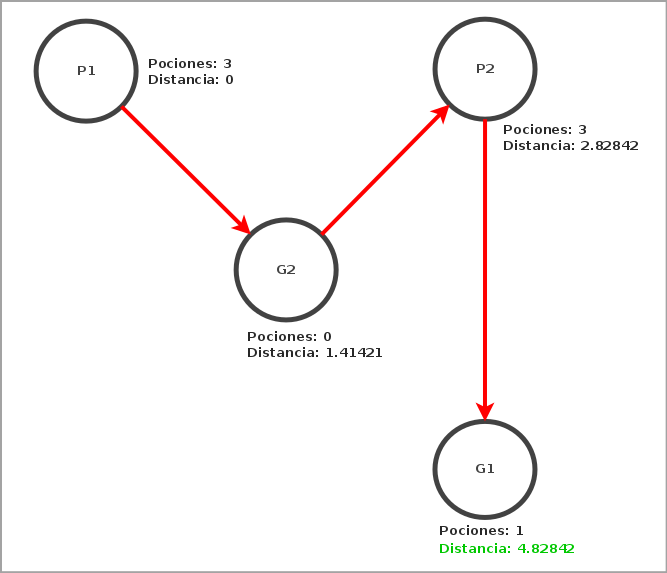
\includegraphics[width=\linewidth]{img/ejercicio1/ejercicio1_ejemplo_camino1_2.png}
        \caption{Camino válido y solución.}
        \label{fig: ejercicio1_ejemplo_camino1_2}
    \end{subfigure}
    \begin{subfigure}[b]{0.49\textwidth}
        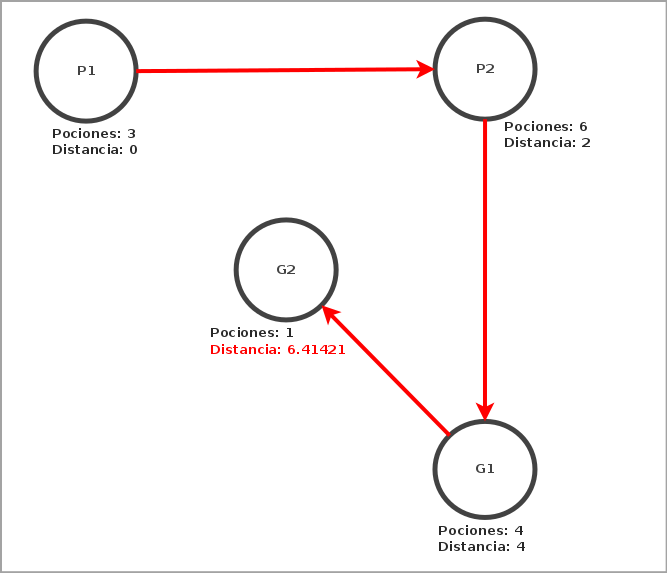
\includegraphics[width=\linewidth]{img/ejercicio1/ejercicio1_ejemplo_camino1_3.png}
        \caption{Camino válido.}
        \label{fig: ejercicio1_ejemplo_camino1_3}
    \end{subfigure}
    \begin{subfigure}[b]{0.49\textwidth}
        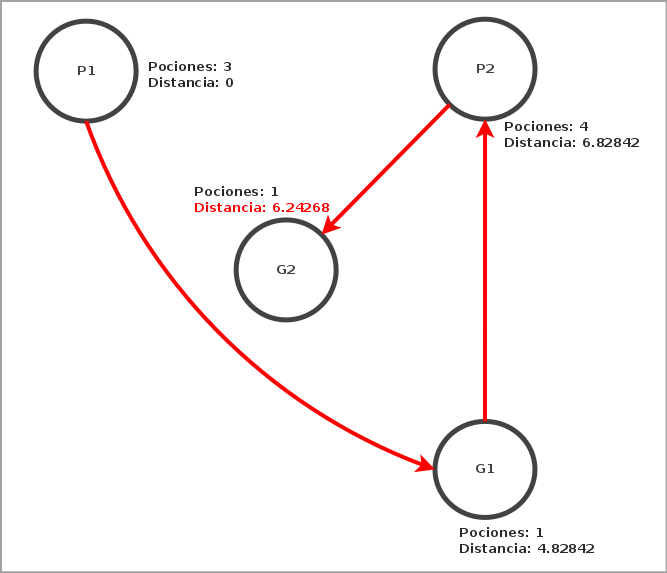
\includegraphics[width=\linewidth]{img/ejercicio1/ejercicio1_ejemplo_camino1_4.png}
        \caption{Camino válido.}
        \label{fig: ejercicio1_ejemplo_camino1_4}
    \end{subfigure}
    \caption{Caminos válidos alcanzados por el algoritmo partiendo del nodo P1. En verde se marcan las distancias mínimas.}
    \label{fig: ejercicio1_ejemplo_caminos1}
\end{figure}

\par El algoritmo, procede a tomar el nodo P2 y calcular todos los caminos que comienzan en él. En la figura \ref{fig: ejercicio1_ejemplo_caminos2} podemos ver todos los caminos válidos que parten del nodo P2. Luego, puede determinar que la distancia mínima es \textbf{4.82842}, y puede tomar como solución cualquiera de los caminos que verificó que dan este resultado.

\begin{figure}[H]
    \begin{subfigure}[b]{0.49\textwidth}
        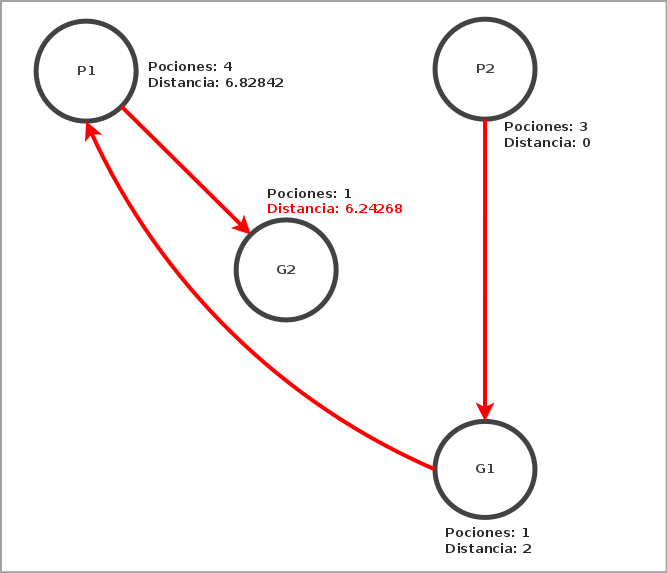
\includegraphics[width=\linewidth]{img/ejercicio1/ejercicio1_ejemplo_camino2_1.png}
        \caption{Camino válido.}
        \label{fig: ejercicio1_ejemplo_camino2_1}
    \end{subfigure}
    \begin{subfigure}[b]{0.49\textwidth}
        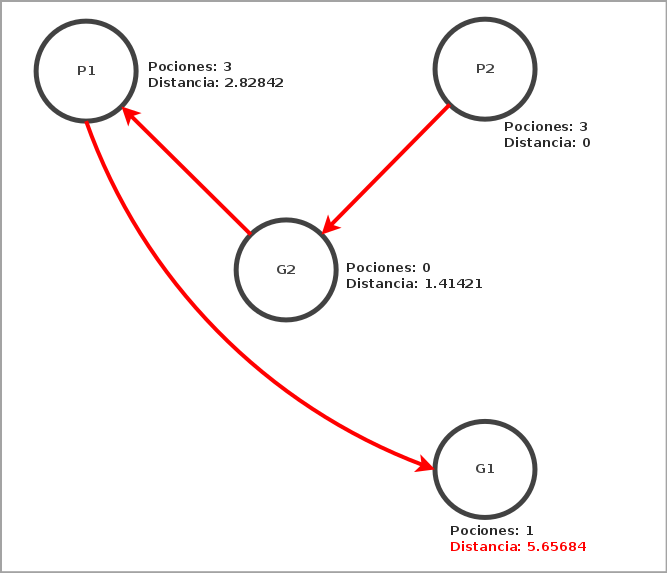
\includegraphics[width=\linewidth]{img/ejercicio1/ejercicio1_ejemplo_camino2_2.png}
        \caption{Camino válido.}
        \label{fig: ejercicio1_ejemplo_camino2_2}
    \end{subfigure}
    \begin{subfigure}[b]{0.49\textwidth}
        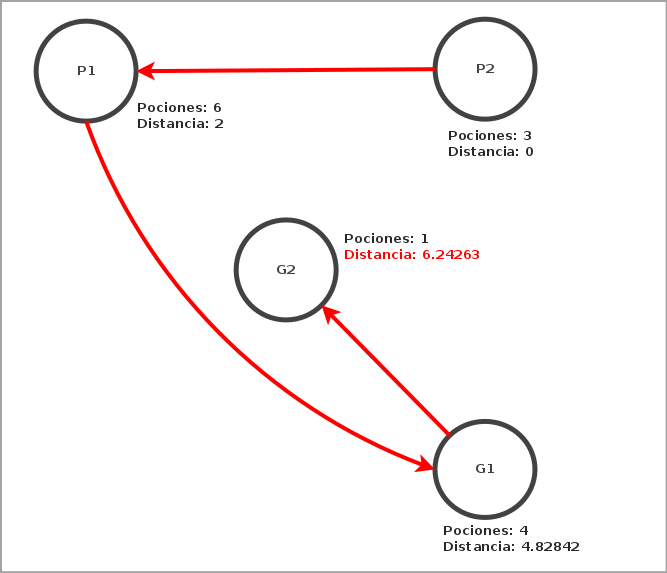
\includegraphics[width=\linewidth]{img/ejercicio1/ejercicio1_ejemplo_camino2_3.png}
        \caption{Camino válido.}
        \label{fig: ejercicio1_ejemplo_camino2_3}
    \end{subfigure}
    \begin{subfigure}[b]{0.49\textwidth}
        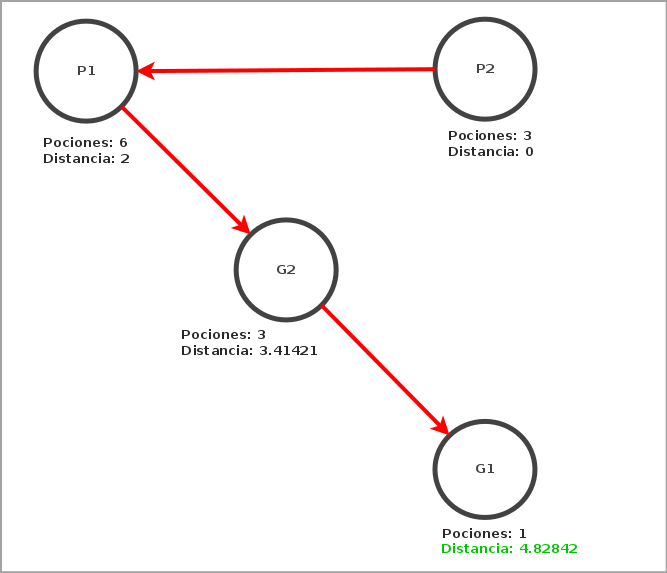
\includegraphics[width=\linewidth]{img/ejercicio1/ejercicio1_ejemplo_camino2_4.png}
        \caption{Camino válido y solución.}
        \label{fig: ejercicio1_ejemplo_camino2_4}
    \end{subfigure}
    \caption{Caminos válidos alcanzados por el algoritmo partiendo del nodo P1. En verde se marcan las distancias mínimas.}
    \label{fig: ejercicio1_ejemplo_caminos2}
\end{figure}

\par Si miramos en detalle las figuras \ref{fig: ejercicio1_ejemplo_camino1_1} y \ref{fig: ejercicio1_ejemplo_camino2_4} podemos ver que ambos caminos llegan al nodo G2 con 3 pociones y solo tienen como no visitado el nodo G1. Por lo que si nos paramos en ese instante, el subproblema pasa a ser saber el camino mínimo partiendo del nodo G2 con 3 pociones y teniendo como nodos a G2 y G1. Luego de definir este subproblema podemos notar que en ambos casos se resuelve de la misma manera este subproblema. En un caso de tamaño muy acotado, como este ejemplo, calcular dos veces un subproblema puede no ser relevante, pero para casos más grandes estos subproblemas repetidos pueden crecer expoencialmente. Para evitar calcular más de una vez un mismo subproblema vamos a definir las instancias: una instancia consta de un nodo en el cual el jugador está parado, una cantidad de pociones que tiene en su mochila y una serie de nodos habilitados para visitar. Una vez calculada una instancia será guardada, lo que nos asegura que al darse otra vez este subproblema podemos recurrir a este valor precalculado y evitar tiempo de procesamiento. más adelante expererimentaremos sobre un algoritmo básico que no tiene en cuenta las instancias y otros que si guardan las instancias (y adoptan otras mejoras) y veremos las diferencias para casos un poco más grandes.

\subsection{Explicación del algoritmo}

\par Para nuestro algoritmo de fuerza bruta utilizamos una función recursiva que se encargue de calcular una instancia. Va a tomar como parámetros:

\begin{itemize}
	\item \textbf{nodo actual:} para identificar la instancia,
	\item \textbf{nodos de tipo parada restantes:} para identificar la instancia,
	\item \textbf{nodos de tipo gimnasio restantes:} para identificar la instancia,
	\item \textbf{pociones en la mochila:} para identificar la instancia,
	\item \textbf{camino recorrida hasta el momento:} para saber si se alcanzó un nuevo camino mínimo o no (sumando la distancia recorrida más el subcamino mínimo calculado en la instancia).
\end{itemize}

\par La función va a llamarse recursivamente para todas las instancias que se desprendan de ella. Por ejemplo, si estamos en un nodo A y podemos pasar al nodo B la función se llamará recursivamente con B como nodo actual, el camino agregando a B al final, actualizando la cantidad de pociones (según corresponda) y quitando a B de los nodos restantes. Veamos un pseudocódigo para entender mejor el funcionamiento.

\par En el pseudocódigo \ref{algo: ejercicio1_pseudocodigo} podemos observar el algoritmo de la función que calcula el camino mínimo dada una instancia del problema. Analicemos su funcionamiento:

\begin{itemize}
	\item Lo primero que se hace es verificar si la instancia ya fué calculada. En ese caso, no se vuelve a calcular y se avanza a devolver esa solución.
	\item Luego se inicializa $solucion$ como inválida. En esta variable se va a guardar la solución (camino mínimo) parcial de la instancia.
	\item Se verifica que queden nodos del tipo gimnasio por recorrer. Recordemos que no es una condición necesaria pasar por todos los nodos de tipo parada, y si se siguiera recorriendo se obtendría un camino mayor, que no sería solución. Si no quedan gimnasios se devuelve un camino con tan solo en nodo actual y distancia 0.
	\item En la linea 8 y 9 se ordenan las listas de nodos restantes por distancia al nodo actual. Esto es una estragia para intentar visitar primero los nodos más cercanos y así lograr alcanzar el camino mínimo más rápido.
	\item Luego se llama recursivamente a la función para cada nodo que pueda ser visitado y se verifica cuál de las soluciones devueltas resulta ser el mínimo de la instancia.
\end{itemize}

\medskip

\SetAlgoLined
\SetKwProg{Fn}{Function}{:}{EndFunction}
\begin{algorithm}[H]
	\label{algo: ejercicio1_pseudocodigo}
	\Fn{calcular\_instancia(camino\_actual: lista(nodo), paradas\_a\_recorrer: lista(nodo), gimnasios\_a\_recorrer: lista(nodo), pociones: int)}{
		\BlankLine
		
		\If{la instancia no fué calculada aún}{
			\BlankLine
			
			$nodo\_actual \gets camino\_actual[|camino\_actual|-1]$\\
			$solucion \gets \O$

			\BlankLine
			\uIf{$| gimnasios\_a\_recorrer | = 0$}{
				\BlankLine
				
				$solucion \gets $camino formado solo por $nodo\_actual$
				
				\BlankLine
			}
			\uElse{
				\BlankLine
				
				ordena $gimnasios\_a\_recorrer$ por distancia a $nodo\_actual$ (de menor a mayor)
				ordena $paradas\_a\_recorrer$ por distancia a $nodo\_actual$ (de menor a mayor)

				\BlankLine
				\For{nodo\_vecino en $gimnasios\_a\_recorrer$}{
					
					\BlankLine
					\If{$pociones \geq pocionesNecesarias(nodo\_vecino)$}{
						\BlankLine

						$subsolucion \gets calcular\_instancia(camino\_actual + nodo\_vecino, paradas\_a\_recorrer, gimnasios\_a\_recorrer - nodo\_vecino, pociones - pocionesNecesarias(nodo\_vecino))$

						\BlankLine
						\uIf{$esValida(subsolucion) \wedge ( \neg esValida(solucion) \vee distancia(subsolucion + nodo\_actual) \leq distancia(solucion) )$}{
							\BlankLine
						
							$solucion \gets subsolucion + nodo\_actual$
						
							\BlankLine
						}
					}
				}

				\BlankLine
				\If{$pociones < mochila$}{
					\BlankLine

					\For{nodo\_vecino en $paradas\_a\_recorrer$}{
						\BlankLine

						$subsolucion \gets calcular\_instancia(camino\_actual + nodo\_vecino, paradas\_a\_recorrer - nodo\_vecino, gimnasios\_a\_recorrer, pociones + 3)$

						\BlankLine
						\uIf{$esValida(subsolucion) \wedge ( \neg esValida(solucion) \vee distancia(subsolucion + nodo\_actual) \leq distancia(solucion) )$}{
							\BlankLine
						
							$solucion \gets subsolucion + nodo\_actual$
						
							\BlankLine
						}
					}
				}
			}
			\BlankLine

			$instancia\_actual \gets solucion$
			\BlankLine
		}
		\BlankLine
		
		\Return $instancia\_actual$
		
		\BlankLine
	}
	\caption{Función encargada de calcular el valor asignado al exponente pasado como parámetro, según el número pasado por parámetro.}
\end{algorithm}



\subsection{Podas y Estrategias}

\par Al tratarse de una algoritmo de fuerza bruta, los tiempos de ejecución suelen ser muy grandes. Por esto, suelen adoptarse estrategias para tratar de disminuirlos. A continuación vamos a explicar las distintas estrategias y podas que se implementaron para este problema.

\par En primer lugar, el diseño del algoritmo se basa fuértemenete en las \textit{instancias} antes mencionadas. La idea es que si ya se calculó una instancia, no vuelva a calcularse. A partir de esto, se podan una enorme cantidad de ramas de cálculo. El problema que surje a partir de esto es que las instancias dependen de los nodos restantes, y no del camino recorrido. Por ende, el hecho de contar con una cota de camino mínimo no te permite podar el cálculo de una instancia. Por ejemplo, supongamos que tenemos 5 nodos: \textit{A, B, C, D, E}. Si debemos calcular la instancia donde el nodo actual es C y los nodos restantes son D y E (sin tener en cuenta las pociones ni los tipos de nodo), no podemos diferenciar si el camino para llegar a C fue A,B o B,A. Por esto, no podemos cortar el cálculo de la instancia por la distancia del camino previo, ya que si se llega a la misma instancia con otro camino previo el resultado puede ser mejor, o hasta incluso la solución del problema. Esto nos limita bastante a la hora de implementar podas que disminuyan los tiempos de ejecución.

\par En cuanto a estrategias tomadas, podemos mencionar:

\begin{itemize}
	\item chequear que la distancia a un nodo al que vamos a ir sea menor que la distancia mínima calculada hasta el momento. De esta manera podemos asegurar que no hay ninguna forma de que nos sirva ir a ese nodo en busca del camino mínimo.
	\item al igual que el caso anterior, pero con el camino mínimo global calculado hasta el momento.
	\item ordenar los gimnasios por la distancia al nodo actual, de menor a mayor. La idea de esta estrategia es que nos conviene ir a los nodos que tenemos más cerca. Es una idea basada en un algoritmo goloso, tratar de ir primero a lo más cercano, y así conseguir un camino menor.
	\item al igual que el caso anterior, pero con los nodos de tipo parada.
	\item visitar primero los nodos del tipo gimnasio. Esta es otra idea basada en un algoritmo goloso, ya que uno quiere visitar todos los nodos del tipo gimnasio en la menor distancia. Entonces se intenta ir primero a nodos de tipo gimnasio.
	\item no recorrer más nodos si ya se han recorrido todos los del tipo gimnasio. El problema pide recorrer todos los gimnasios, pero no es necesario recorrer el resto. Por esto, una vez que se han recorrido todos los gimnasios no se continúa.
	\item si la mochila del jugador se encuentra llena, no se recorren más paradas. Si no hay capacidad para guardar más pociones, no sirve de nada visitar más nodos del tipo parada, ya que eso implicaría más distancia (por la desigualdad triangular).
	\item se realiza un goloso para tener una cota inicial. De esta manera, se tiene un camino mínimo parcial para ser utilizado como cota.
\end{itemize}

\par más adelante, en la sección de Experimentación (Sección \ref{subsec: ejercicio1_experimentacion}), se analizarán las distintas estrategias y podas y se verá su comportamiento con distintos tipos de entrada en función del tiempo de ejecución y otras variables.



\subsection{Análisis de complejidad}

\par Para analizar la complejidad del algoritmo y su implementación debemos definir ciertos conceptos y parámetros:

\begin{itemize}
	\item \textbf{n}: Cantidad de nodos del tipo gimnasio.
	\item \textbf{m}: Cantidad de nodos del tipo parada.
	\item \textbf{k}: Capacidad de la mochila del jugador.
\end{itemize}

\par A continuación vamos a ver las partes importantes y relevantes del algoritmo y analizaremos la complejidad. Primero, veamos la función $calcular\_instancia$.

\begin{itemize}
	\item Calcular el número de instancia es O($n+m$). Esto porque se arma un número binario con la posición $N_i$=1 si el nodo $i$ está en la instancia o $N_i$=0 si no y luego se pasa de binario a decimal. Es importante tener en cuenta también que se deben calcular potencias de 2.
	\item Ordenar los nodos de tipo parada cuesta O($m^2$).
	\item Ordenar los nodos de tipo gimnasio cuesta O($n^2$).
	\item Tanto calcular la distancia como copiar el vector $gimnasios\_a\_recorrer$ cuesta O($n$) y se realiza para cada nodo en el vector $gimnasios\_a\_recorrer$. Entonces nos queda O($n^2$).
	\item Calcular la distancia cuesta y copiar el vector $paradas\_a\_recorrer$ cuesta O($n+m$) y se realiza para cada nodo en el vector $paradas\_a\_recorrer$. Entonces nos queda O($m \cdot (n+m)$).
	\item En total, tenemos que la función $calcular\_instancia$ cuesta O($n+m + m^2 + n^2 + m^2 + m \cdot (n+m)$) = O($n^2 + m^2 + n \cdot m$) = \textbf{O($\boldsymbol{n^2 + m^2}$)}.
\end{itemize}

\par Tenemos entonces que la función $calcular\_instancia$ cuesta O($n^2 + m^2$). Recordemos que esta función se utilizaba para para calcular una instancia, y nunca calcula dos veces la misma instancia. Veamos entonces la cantidad màxima de instancias. Una instancia se diferenciaba por:

\begin{itemize}
	\item \textbf{nodo actual}: la cantidad máxima de nodos es $n+m$.
	\item \textbf{pociones}: la cantidad máxima de pociones està acotada por la capacidad de la mochila: $k$.
	\item \textbf{nodos restantes}: el número binario de instancia tiene longitud $n+m$ (una posición por cada nodo). Al pasarlo a entero, tenemos $2^{n+m}$. Porque el número máximo sería el que tiene todas las posiciones en 1: $\sum_{i=0}^{n+m-1}2^i$ = $2^{n+m}-1$. Tengamos en cuenta que iniciamos a contar en 0. Entonces de 0 a $2^{n+m}-1$ tenemos $2^{n+m}$ números.
\end{itemize}

\par De esta manera vemos que tenemos $(n+m) \cdot k \cdot 2^{n+m}$ posibles instancias. En general, se calcularán muchas menos instancias, pero existen casos donde se calcula esa cantidad, por lo que es una cota superior.

\par Tenemos entonces que la función $calcular\_instancia$ cuesta O($n^2 + m^2$) y puede llegar a ejecutarse $(n+m) \cdot k \cdot 2^{n+m}$ veces. Por lo tanto esta implementación tiene una complejidad O($(n^2 + m^2) \cdot (n+m) \cdot k \cdot 2^{n+m}$). Veamos mejor la primera parte de esta cota: $n^2 + m^2 \cdot (n+m)$.

\begin{equation}
	(n^2 + m^2) \cdot (n+m) = n^3 + n^2 \cdot m + m^3 + m^2 \cdot n
\end{equation}

Si $n > m$, tenemos que O($n^3 + n^2 \cdot m + m^3 + m^2 \cdot n$) = O($n^3$). Si en cambio $m > n$, tenemos que O($n^3 + n^2 \cdot m + m^3 + m^2 \cdot n$) = O($m^3$). Si en cambio, $n = m = l$, tenemos que O($n^3 + n^2 \cdot m + m^3 + m^2 \cdot n$) = O($l^3$). Por esto, podemos decir que O($n^3 + n^2 \cdot m + m^3 + m^2 \cdot n$) = O($n^3 + m^3$). Entonces volviendo a la complejidad del problema nos queda \textbf{O($\boldsymbol{(n^3 + m^3) \cdot k \cdot 2^{n+m}}$)}.



\subsection{Experimentación}
\label{subsec: ejercicio1_experimentacion}

\par Antes de comenzar la experimentación, vamos a definir las distintas versiones del programa:

\begin{itemize}
	\item \textbf{Versión 0}:
		\begin{itemize}
			\item No almacena las instancias calculadas, por lo cual puede calcular más de una vez el mismo subcamino.
			\item Intenta ir siempre primero a los gimnasios.
			\item No va a una parada si no tiene capacidad para almacenar nuevas pociones.
			\item No va a más paradas si no quedan gimnasios por recorrer.
		\end{itemize}
	\item \textbf{Versión 1}:
		\begin{itemize}
			\item Incluye todas las estrategias y podas de la versión 0.
			\item Almacena las instancias calculadas.
		\end{itemize}
	\item \textbf{Versión 2}:
		\begin{itemize}
			\item Incluye todas las estrategias y podas de la versión 1.
			\item Verifica que la distnacia al siguiente nodo (al cual va a moverse) no supere la distancia mínima parcial (de su misma instancia).
			\item Verifica que la distnacia al siguiente nodo (al cual va a moverse) no supere la distancia mínima parcial global (de todas las instancias).
		\end{itemize}
	\item \textbf{Versión 3}:
		\begin{itemize}
			\item Incluye todas las estrategias y podas de la versión 2.
			\item En cada instancia, ordena los gimnasios según la distancia al nodo actual (de menor a mayor). Con esto intenta ir primero a los gimnasios más cercanos.
			\item En cada instancia, ordena las paradas según la distancia al nodo actual (de menor a mayor). Con esto intenta ir primero a las paradas más cercanas.
		\end{itemize}
	\item \textbf{Versión 4}:
		\begin{itemize}
			\item Incluye todas las estrategias y podas de la versión 3.
			\item Al comenzar la ejecución, corre una heurística golosa. Conserva este resultado como cota superior.
		\end{itemize}
\end{itemize}

\par La versión 0 nos servirá de guía para ver cuánto influye el almacenamiento de instancias en los tiempos de ejecución. Luego veremos en cada versión cuanto influye la incorporación de cada poda y estrategia en los tiempos de ejecución.

\par A continuación se correrán distintos casos con ciertas características para ver el comportamiento de las distintas versiones del programa.

\subsubsection{Experimento 1: Cantidad de paradas vs Tiempos de ejecución}

\par En el primer experimento vamos a analizar los tiempos de ejecución en función de la cantidad de paradas. Para esto, vamos a dejar fija la cantidad de gimnasios y la capacidad de la mochila, iremos aumentando la cantidad de paradas y veremos cómo se comportan los tiempos de ejecución.

\par Tomaremos \textit{cantidad de gimnasios = 3} y \textit{capacidad de la mochila = 5}. Vamos a comenzar con \textit{cantidad de paradas = 1} y la iremos aumentando hasta llegar a 15. Generaremos los casos de entrada de forma aleatoria, respetando los parámetros y verificando que tengan solución.

\par Esperamos ver una gran diferencia entre la Versión 0 y las restante, ya que va a calcular muchas instanncias repetidas veces y el resto no. Entre las otras, no esperamos ver gran diferencia, pero nos gustaría que con mas estrategias y podas mejoren los tiempos.

\begin{figure}[H]
	\begin{center}
		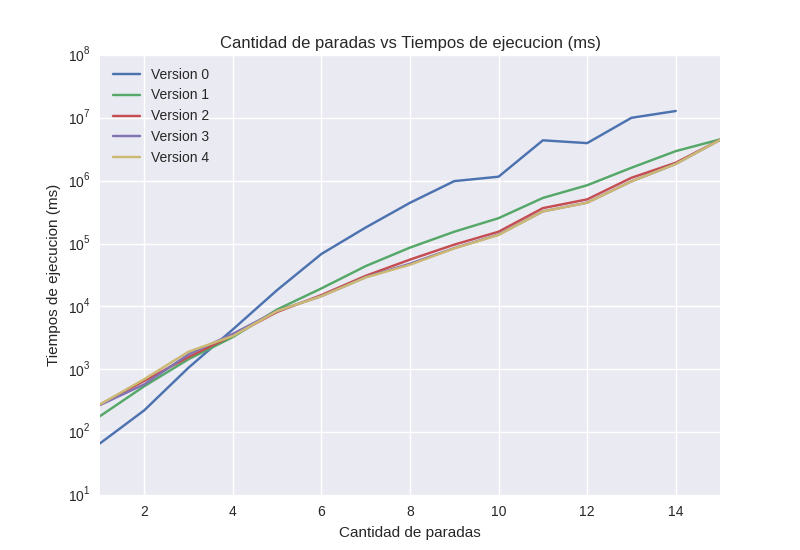
\includegraphics[width=\textwidth]{img/ejercicio1/exp1_1.png}
		\caption{Resultados del experimento 1.}
		\label{fig: ej1_exp1_1}
	\end{center}
\end{figure}

\par En la figura \ref{fig: ej1_exp1_1} podemos ver los resultados del experimento 1. Como esperábamos, la versión 0 cuenta con los tiempos más altos y supera al resto ampliamente (teniendo en cuenta que el gráfico se muestra con escala logarítima). En un comienzo, la versión 0 toma menos tiempo de procesamiento, porque los casos de entrada son muy pequeños e influye mucha inicializar la estructura de instancias. Pero a partir de 4 paradas se ve como se desprende del resto y se eleva con mucha más rapidez.

\par Para poder ver mejor los resultados de las versiones 1, 2, 3 y 4, en la figura \ref{fig: ej1_exp1_2} se excluyó a la versión 0 y se centró el foco en las cantidad de paradas mayores a 8. Podemos ver que no se toman grandes diferencias. También es interesante que entre la versión 3 y la 4 no se sacan diferencias. Creemos que esto se debe a que a partir de una cierta cantidad de paraadas el cálculo de la herística golosa deja de influir. Podemos decir entonces que en cuanto a la cantidad de paredes, nos conviene quedarnos con la versión 3 ó 4.

\begin{figure}[H]
	\begin{center}
		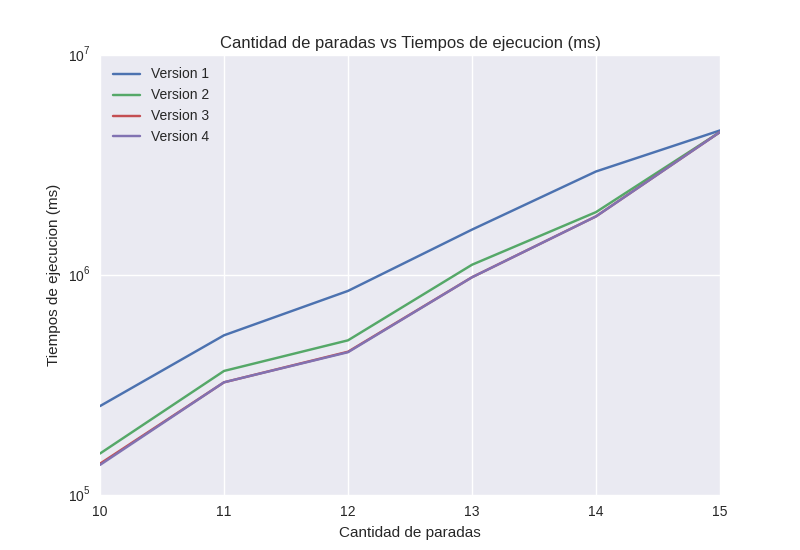
\includegraphics[width=\textwidth]{img/ejercicio1/exp1_2.png}
		\caption{Resultados del experimento 1 ampliado en las cantidades de paradas mayores a 8 y excluyendo la versión 0.}
		\label{fig: ej1_exp1_2}
	\end{center}
\end{figure}


\subsubsection{Experimento 2: Cantidad de gimnasios vs Tiempos de ejecución}

\par En este experimento vamos a analizar los tiempos de ejecución en función a la cantidad de gimnasios. Vamos a fijar los parámetros \textit{cantidad de paredes} y \textit{capcidad de la mochila} y veremos como se comportan las distintas versiones del programa.

\par Tomaremos \textit{cantidad de paredes = 4} y \textit{capacida de la mochila = 4}. Iremos aumentando \textit{cantidad de gimnasios} desde 1 hasta 10 y generaremos una serie de casos aleatorios respetando los parámetros. Los casos de entrada se generan de forma tal que siempre exista solución al problema.

\par Esperamos nuevamente que la versión 0 se encuentre lejana al resto. No creemos que las otras versiones se distancien mucho entre sí, ya que todas intentan primero ir a un gimnasio, por lo que no van a podar mucho estos caminos.

\begin{figure}[H]
	\begin{center}
		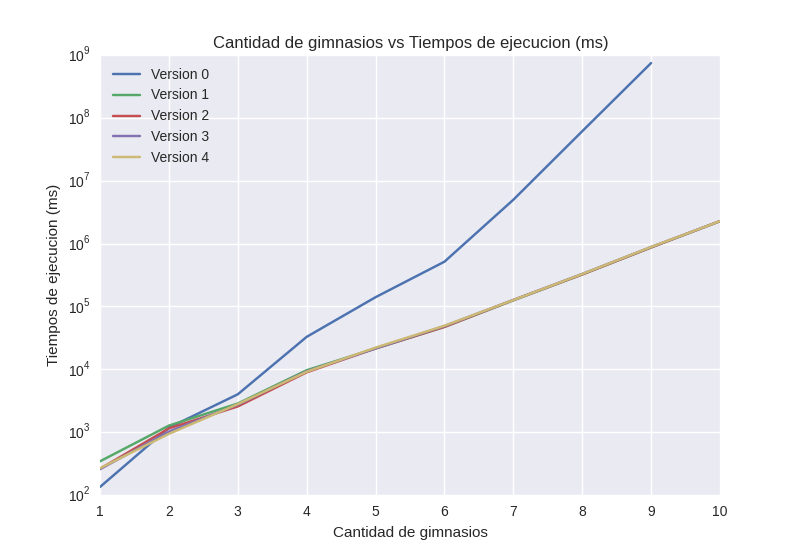
\includegraphics[width=\textwidth]{img/ejercicio1/exp2_1.png}
		\caption{Resultados del experimento 2.}
		\label{fig: ej1_exp2_1}
	\end{center}
\end{figure}

\par Podemos ver en la figura \ref{fig: ej1_exp2_1} los resultados del experimento. Vemos que se cumple lo que esperábamos sobre la versión 0 y notamos que las versiones 1, 2, 3 y 4 se encuentran casi superpuestas.




\subsubsection{Experimento 3: Capacidad de la mochila vs Tiempos de ejecución}

\par En este experimento vamos a variar la capacidad de la mochila y analizar el comportamiento de las versiones del programa. Dejaremos fijos los parámetros \textit{cantidad de paradas} y \textit{cantidad de gimnasios} y analizaremos los tiempos de ejecución de cada versión en base al parámetro \textit{capacidad de la mochila}.

\par Aquí también se espera que la versión 0 tenga tiempos de ejecución mayores al resto. Viendo los resultados de los experimentos previos, no esperamos grandes diferencias entre los restantes, ya que la condición a la que afecta la capacidad de la mochila es si puedo ir a un gimnasio o no, y esta condición afecta a todas las versiones por igual.

\par Para llevar a cabo el epxerimento vamos a tomar \textit{cantidad de gimnasios = 4} y \textit{cantidad de paradas = 4} e iremos aumentando el parámetro \textit{capacidad de la mochila} desde 1 hasta 10. Los casos de entrada serán generados de la misma forma que los dos experimentos previos.

\begin{figure}[H]
	\begin{center}
		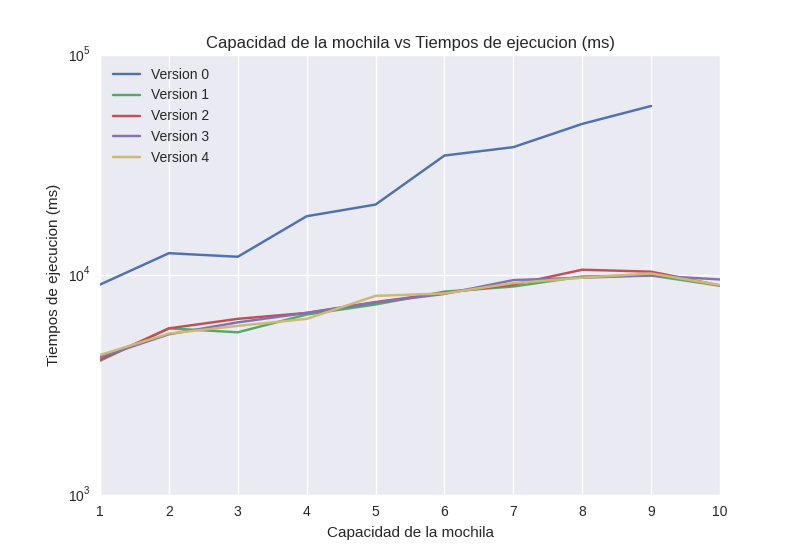
\includegraphics[width=\textwidth]{img/ejercicio1/exp3_1.png}
		\caption{Resultados del experimento 3.}
		\label{fig: ej1_exp3_1}
	\end{center}
\end{figure}

\par En la figura \ref{fig: ej1_exp3_1} podemos ver los resultados del experimento 3. Podemos ver que las podas hacen que las versiones 1, 2, 3 y 4 mejores mucho los tiempos de ejecución. Pero también notamos que no se observan grandes diferencias entre ellas. Ninguna versión se acomoda por debajo del resto en cuanto a tiempos de ejecución.

\par Ninguno de los 3 experimentos nos dio un resultado desfavorable para la versión 4. Por lo que creemos que lo mejor es utilizar esta versión que incluye una cota de heurística golosa y no parece ser influyente en los tiempos de ejecución.


\subsubsection{Experimento 4: Pociones necesarias para los gimnasios - TSP vs no-TSP}

\par Hasta el momento siempre tomamos casos donde el jugador necesitaba pociones para ir a los gimnasios. Pero un caso particular es cuando no necesita pociones para ir a ningún gimnasio, por lo cual no necesita visitar paradas. En este caso, el problema termina siendo calcular la distancia mínima que se debe recorrer para visitar todos los nodos del tipo gimnasio. Este problema es conocido como `El problema del viajante de comercio' (TSP: Traveling Salesman Problem).

\par En este experimento, vamos a tratar ese caso particular. Por lo que vamos a variar el parámetro $Pociones necesarias para un gimnasio$ entre 0 y 3. El caso en que valga 0 va a ser el caso de TSP. Queremos ver como se comporta el algoritmo para este caso particular y determinar si se trata de un mejor o peor caso o si no se diferencia del resto. Por el diseño del algoritmo, siempre se comienza por un nodo del tipo parada. Por lo que siempre vamos a dejar un nodo del tipo parada (aunque se trate de un TSP y solo se necesiten gimnasios).

\par Para esto vamos a fijar el parámetro $Capacidad de la mochila$ y vamos a comenzar con 2 nodos e iremos aumentando esta cantidad de a 2. Dependiendo si se trata de el caso TSP o no tomaremos distintas determinaciones:

\begin{itemize}
	\item \textbf{TSP}: siempre habrá un nodo de tipo parada y el resto de tipo gimnasio.
	\item \textbf{no-TSP}: tomaremos $Cantidad de paradas = Cantidad de gimnasios = \frac{nodos}{2}$.
\end{itemize}

\par Para cada caso, generamos los nodos (y sus ubicaciones) y se le aplicó un valor distinto al parámetro $Pociones necesarias para un gimnasio$ dependiendo el caso. Inclusive, se modificó la cantidad de paradas o gimnasios. Pero no así las ubicaciones, por lo que siempre se utilizan los mismos nodos.

\begin{figure}[H]
	\begin{center}
		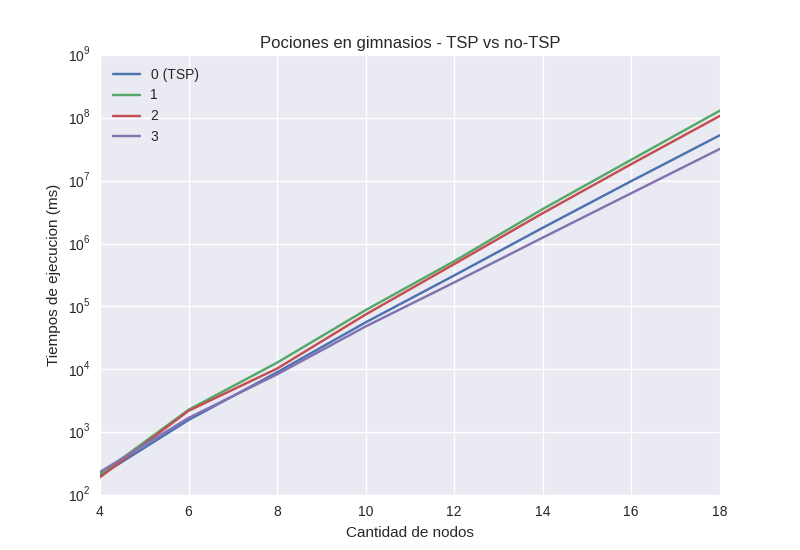
\includegraphics[width=\textwidth]{img/ejercicio1/exp5_1.png}
		\caption{Resultados del experimento 4.}
		\label{fig: ej1_exp5_1}
	\end{center}
\end{figure}

\par En la figura \ref{fig: ej1_exp5_1} podemos ver los resultados del experimento 4. Podemos notar que el caso TSP y el caso con 3 $Pociones necesarias$ se diferencian de los otros dos casos, tomando menor tiempo de ejecución. Notamos que el caso 3 es muy favorable, a diferencia de los 1 y 2. Creemos que esto se debe a que al necesitarse más pociones para ir a los gimnasios se realizan más podas que limitan la cantidad de instancias visitadas. Para esto, vamos a indagar más en el tema y compararemos los siguientes datos:

\begin{itemize}
	\item Cantidad de instancias visitadas: es la cantidad de instancias que se visitaron, sin importar si se calculó este valor o no.
	\item Cantidad de instancias calculadas: es la cantidad de instancias para las cuales se calculó la distancia mínima.
	\item Cantidad de podas del tipo 1: las podas del tipo 1 son: parar si no quedan más gimnasios; no ir a parada si tiene la mochila llena.
	\item Cantidad de podas del tipo 2: las podas del tipo 2 son: si la distancia al siguiente nodo es mayor que la distancia mínima parcial de la instancia no va a ese nodo; si la distancia al siguiente nodo es mayor que la distnacia mínima parcial global no va a ese nodo.
\end{itemize}

\newcolumntype{C}[1]{>{\centering\let\newline\\\arraybackslash\hspace{0pt}}m{#1}}

\begin{table}[h]
	\centering
	\rowcolors{2}{blue!10}{white}
	\begin{tabular}{|C{2cm}|C{2cm}|C{2cm}|C{2cm}|C{2cm}|C{2cm}|}
		\hline
		\rowcolor{gray!30}
		Cantidad de nodos & Pociones Gimnasio &  Cantidad de instancias visitadas &  Cantidad de instancias calculadas &  Cantidad de podas 1 &  Cantidad de podas 2 \\
		\hline
		4 &           0 (TSP) &                              13.0 &                               11.0 &                  2.5 &                  1.5 \\
		\hline
		4 &                 3 &                              20.5 &                               15.5 &                  4.0 &                  1.0 \\
		\hline
		6 &           0 (TSP) &                             160.0 &                               80.5 &                  5.0 &                  5.5 \\
		\hline
		6 &                 3 &                             182.5 &                               90.0 &                 18.0 &                  3.5 \\
		\hline
		8 &           0 (TSP) &                            1345.0 &                              449.0 &                  7.0 &                  7.0 \\
		\hline
		8 &                 3 &                            1258.5 &                              448.0 &                 88.0 &                  1.5 \\
		\hline
		10 &           0 (TSP) &                            9220.0 &                             2305.0 &                  9.0 &                  6.0 \\
		\hline
		10 &                 3 &                            7494.5 &                             2100.0 &                425.0 &                  0.5 \\
		\hline
		12 &           0 (TSP) &                           56309.0 &                            11264.5 &                 11.0 &                 22.5 \\
		\hline
		12 &                 3 &                           41113.0 &                             9504.0 &               1986.0 &                  5.0 \\
		\hline
		14 &           0 (TSP) &                          319431.0 &                            53247.5 &                 13.0 &                 69.5 \\
		\hline
		14 &                 3 &                          213665.5 &                            42042.0 &               9016.0 &                 16.5 \\
		\hline
		16 &           0 (TSP) &                         1720300.0 &                           245760.5 &                 15.0 &                 35.5 \\
		\hline
		16 &                 3 &                         1068495.5 &                           183040.0 &              40048.0 &                  8.5 \\
		\hline
		18 &           0 (TSP) &                         8912894.0 &                          1114113.0 &                 17.0 &                 20.0 \\
		\hline
		18 &				 3 &                         5191762.0 &                           787644.0 &             175041.0 &                  5.0 \\
		\hline
	\end{tabular}
	\caption{Datos de las corridas de casos TSP vs casos 3 pociones.}
	\label{tab: ej1_exp5_2}
\end{table}

\par En el cuadro \ref{tab: ej1_exp5_2} podemos ver los datos de las corridas de cada caso de entrada. Notamos que, para cualquier cantidad de nodos de entrada, la cantidad de instancias visitadas y la cantidad de instancias calculadas difieren mucho entre TSP y no-TSP. Este se condice diréctamente con la diferencia que se ve en la cantidad de podas del tipo 1. Esto se lo adjudicamos al hecho de que, para el caso de TSP, todos los nodos son de tipo gimnasio (excepto el primero). Por esto, no se realiza ninguna poda, todo camino es válido. Mientras que en el caso de no-TSP, se realizan muchas podas por no tener pociones suficientes para ir a algún gimnasio.

\par Finalmente, podemos comprender el por qué de las diferencias a favor del caso con $pociones necesarias = 3$. Vemos entonces que el caso TSP es simplemente un caso más, y no se trata de un mejor ni peor caso.

\medskip

\par De esta manera podemos concluir que estamos conformes con la forma en que pudimos disminuír los tiempos de ejecución del algoritmo, pero creemos que se podría haber probado una versión sin instancias, y que tenga libertad de podar teniendo en cuenta el camino previo (algo que la instancia planteada no nos permite).